\chapter{Proportional reasoning}
\label{ch:proportions}

\chapquote{Give me the place to stand, and I shall move the earth.}{Archimedes, Ancient Greek mathematician and philosopher}

A key concept in pre-algebra mathematics is proportionality. The ideas of ratio, proportion, and percent are probably familiar to you, and you likely have solved proportions in your mathematical career so far.

In this chapter we will apply the tools and techniques we learned in \cref{ch:equations} to some of these familiar contexts. Then we will take proportionality to the ``algebra level'' by exploring the concepts of direct and inverse variation.

% % % % % % % % % % % % % % % % % % % % % % % % % % % % % % % % % % % % % % % % 
\section{Proportions as equations}
\label{sec:propsaseqs}

Mathematicians, like Yeardleigh's team of gourmet chefs, won't use tools, techniques, or ingredients unless they know exactly where they come from. This is the attitude we adopt, for the most part, in algebra. This point of view, however, may upset some students' mathematical status quo.

Case in point: solving proportions. Many of us have been taught a mysterious method called ``cross multiplication'' as a means of solving a proportion. Unless we can explain it's inner workings -- Where does it come from? Why does it give us the correct answer? -- then the technique must be considered off-limits.

We'll explain so-called cross-multiplication in this chapter, and explore alternative (easier) methods of handling proportions.

%\begin{boxexplore}[Extended exploration: Multiply and conquer]
%\addtodoitem{Click here to visit the extended exploration: Multiply and Conquer}
%\end{boxexplore}
\addtodoitem{Link to extended exploration: Multiply and conquer}

\begin{boxexplore}[Hamster and superhamster]
Genetic engineers at YeardleighCorp have genetically engineered superhamsters that weigh 15 ounces. Tests indicate that one superhamster can carry a 40-ounce packet of food on its back. If a human could carry the same amount as a superhamster, relative to body mass, how many pounds could a 120-pound teenager carry?
\end{boxexplore}

\kverse{YeardleighCorp genetic engineers develop super-hamster.}

We have mentioned that the study of mathematical relationships is a central idea of algebra. One helpful skill for studying relationships is the ability to make sound mathematical comparisons.

\begin{boxdef}[Ratio]
A comparison of two quantities, often expressed as a fraction.
\end{boxdef}

There are two main types of ratios: part-to-part ratios and part-to-whole ratios. For example, ``number of girls in class to number of boys in class'' is a part-to-part ratio, whereas ``number of girls in class to number of students in class'' is a part-to-whole ratio.

\begin{boxdef}[Proportion]
An equation stating that two ratios are equal.
\end{boxdef}

Proportions are just equations, and so we don't need any special techniques like ``cross-multiplication'' to solve them. We can use the trusty properties of equality, just as we do with any other equation.

\begin{boxex}
Solve for $x$: $\dfrac{x}{15}=\dfrac{44}{60}$

\exsoln\ Our suggestion is not to think of the left side as a fraction at all. Think of it as $x$ divided by 15. That's just a Level 1 linear equation! We need to get rid of the ``divide by 15'' and so we multiply both sides by 15.
\[\begin{aligned}
15\cdot\frac{x}{15} &= 15\cdot\frac{44}{60}\\[2ex]
\cancel{15}\cdot\frac{x}{\cancel{15}} &= \cancel{15}\cdot\frac{44}{\cancel{15}\cdot4}\\[2ex]
x&=11
\end{aligned}\]
After a bit of simplifying, we have isolated $x$ with just one application of MPOE.
\end{boxex}

We call this approach ``clear the denominator''. Of course, it's not the only way to solve a proportion, and not always the easiest way.\footnote{You may have learned other approaches for solving proportions, and that's a good thing! One very handy approach is to scale up (or down) one (or both) of the ratios so that they have a common numerator or denominator: another application of the identity property of multiplication!}

\subsection{Adding a bit more complexity}

In their most basic form, proportions have the unknown in the numerator of one of the ratios. These are just Level 1 (one-step) equations. All we need to do to solve them is multiply both sides of the equation by the denominator of the unknown (that's MPOE in action).

But what if the unknown is in the denominator of a fraction?

\begin{boxex}
The startup exploration problem says that a 15-ounce superhamster can carry a 40-ounce packet of food on its back. At that rate of strength, how many pounds could a 120-pound teenager carry?

\exsoln\ Let's write a proportion comparing the ratio of weight to carrying capacity, and let us use $P$ to represent the amount that the teenage can carry, in pounds. Then we have: \[\frac{15 \text{ ounces}}{40 \text{ ounces}} = \frac{120 \text{ pounds}}{P \text{ pounds}}\]

We wrote these ratios as ``weight/carrying capacity'', but of course we could also  have written the ratios as ``carrying capacity/weight''. So, one solution approach is to take the reciprocal of both sides. That will put the unknown conveniently in the numerator!
\[\begin{aligned}
\frac{40 \text{ ounces}}{15 \text{ ounces}} &= \frac{P \text{ pounds}}{120 \text{ pounds}}
\\[2ex]
120\cdot\frac{40}{15} &= 120\cdot\frac{P}{120}
\\[2ex]
320 &= P
\end{aligned}\]
So, a 120-pound teenage of superhamster strength could carry 320 pounds of food. For comparison, according to the US census, the average American ate approximately 257 pounds of fruit in 2009 (including fresh fruit, dried fruit, and fruit juice). So this teenager could carry 25\% more fruit than they would typically eat in a year.
\end{boxex}

Very often in mathematical comparisons, it is helpful to create a comparison ``per unit'' of some quantity: miles \textit{per hour}, dollars \textit{per pound}, and so on. These ``per unit'' comparisons mean ``per \textit{one} unit''. For example, if Bob buys 3 pounds of Swiss cheese for \$19.50, then we can find an equivalent ratio \[\frac{19.50}{3} = \frac{6.50}{1}\] and see that the cheese costs ``6.50 dollars per (one) pound''.

\begin{boxdef}[Unit rate]
A \gls{unit rate} is a ratio in which the value of one of the quantities is 1. For example ``miles per hour'', meaning ``miles traveled in \textit{one} hour''.
\end{boxdef}

Before we move on, the maneuver we made in the last example --- taking the reciprocal of both sides --- bears another moment of reflection.

\begin{boxdef}[Tangent: Explaining reciprocal of both sides]
Is ``take the reciprocal of both sides'' a property of equality? In other words, if we know that $a = b$, do we know for sure that $\frac{1}{a} = \frac{1}{b}$ is always true?

The fact that $a$ and $b$ end up in the denominator of a fraction means that we must require that $a$ and $b$ are non-zero at the start. If $a$ and $b$ are both non-zero, then we can use DPOE with both numbers.
\[\begin{aligned}
a &= b
&&\text{\quad We assume that this is true, and that $a$ and $b$ are non-zero}
\\[2ex]
\frac{a}{a} &= \frac{b}{a}
&&\text{\quad DPOE, using $a$}
\\[2ex]
1 &= \frac{b}{a}
&&\text{\quad Simplify}
\\[2ex]
\frac{1}{b} &= \frac{b}{a\cdot b}
&&\text{\quad DPOE, using $b$}
\\[2ex]
\frac{1}{b} &= \frac{\bcancel{b}}{a\cdot \bcancel{b}}
&&\text{\quad Cancel the common factor}
\\[2ex]
\frac{1}{b} &= \frac{1}{a}
&&\text{\quad Voil\`a}
\end{aligned}\]
So, in the end, if two numbers (both nonzero) are equal, then we know that their reciprocals are equal as well. ``Take the reciprocal of both sides'' is a property of equality.
\end{boxdef}

Of course, we might be faced with numerators and denominators that are more complicated. Here's an example with variables on both sides of the equation. Our approach is to use MPOE to clear \textit{both of the denominators}.

\begin{boxex}
Solve for $x$: $\dfrac{x+1}{2}=\dfrac{x+2}{5}$

\exsoln\
\[\begin{aligned}
\dfrac{x+1}{2} &=\dfrac{x+2}{5}
\\[2ex]
\bcancel{2}\cdot5\cdot\left(\frac{x+1}{\bcancel{2}}\right) &=
2\cdot\cancel{5}\cdot\left(\frac{x+2}{\cancel{5}}\right)
&&\quad\text{MPOE two times!}
\\[2ex]
5(x+1) &= 2(x+2)
\\
5x+5 &= 2x+4
&&\quad\text{distributive property}
\\
3x &= 1
&&\quad\text{SPOE two times!}
\\[2ex]
x &= \dfrac{1}{3}
&&\quad\text{DPOE}
\end{aligned}\]
To write our answer in set notation, we have $\solset{\frac{1}{3}}$.
\end{boxex}

The previous example may give you some insight into how cross-multiplication works, and might come in handy when working on the problems and exercises.

\begin{boxwarn}
Solve: $\dfrac{x+2}{5} = \dfrac{7}{6}$

There may be a temptation to subtract 2 from both sides in the first step. \[\dfrac{x+2-2}{5} = \frac{7-2}{6} \qquad\implies\qquad \dfrac{x}{5} = \frac{5}{6}\]
But, to do so would be \evilandwrong! The x+2 is grouped together by the fraction bar (vinculum) and that little group is divided by 5. Before we can manipulate the group, we have to undo the division by 5. Then, the 2 is free to be subtracted.

Note that this is the same kind of structure as \[ 4(x+2) = 16\] Here we have to divide both sides by 4, before we can use SPOE on the $x+2$. For some reason the temptation to subtract first is stronger when in fraction form (maybe because the grouping isn't obvious without the parentheses). In any case: beware!
\end{boxwarn}

% % % % % % % % % % % % % % % % % % % % % % % % % % % % % % % % % % % % % % % % 
\section{Applications of proportional reasoning}
\label{sec:probsolvwithprops}

Proportional reasoning encompasses a key set of skills that are important to have in your problem solving toolbox. In this section we'll discuss a few of the classic ways that ratio and proportion show up in problem solving contexts.

\subsection{Percent}

\kverse{Bob owns a lot of Spam.}

\begin{boxexplore}[Spam ``less'' sodium]
Bob is counting cans of Spam in his pantry. For every 3 cans of ``low-sodium'' Spam, he has 5 cans of Spam with the usual (higher) amount of sodium. What percent of the Spam in his pantry is low-sodium? 
\end{boxexplore}

Break the word ``percent'' into its component parts, ``per cent'', and think about what each part means. The word ``cent'' indicates 100 (there are 100 {\em} cents in a dollar, and 100 years in a \textit{cent}ury), while the word ``per'' indicates that we are making a comparison (earning \$10 \textit{per} hour at a job means you earn \$10 for every hour that you work).

Putting the words back together, percent means ``per 100'' or ``for every 100''. When we write a percent as 75\%, or say out loud ``seventy-five percent'', we're really mean ``75 per 100'' or ``75 out of 100''. We could write the decimal 0.75, or the fraction $\frac{75}{100}$.

The fraction $\frac{75}{100}$ isn't in lowest terms, so we could write instead: \[\frac{3}{4} = \frac{75}{100}\]
Proportion is the heart of percent, and percent problems are all really about the percent proportion: \[\frac{\text{part}}{\text{whole}} = \frac{\text{percent}}{100}\]
So given a percent question, we just have to ask ourselves which pieces of the percent proportion we know, and which we are trying to find.

\begin{boxex}
Write proportions that could be used to solve each of the following:
\begin{enumerate}
	\item What number is 10\% of 20?
	\item What percent of 75 is 50?
	\item 15 is 25\% of what number?
\end{enumerate}

\expsoln
\begin{enumerate}
	\item \onerowex{$\dfrac{x}{20}=\dfrac{10}{100}$}{We're given the percent (10\%) and the whole (20). The word ``of'' is one hint that 20 is the whole. We're looking for the percent, so that's where we'll write the unknown ($x$, or whatever variable you like). Solve the proportion for the unknown, and we'll have our answer.}

	\item \onerowex{$\dfrac{50}{75}=\dfrac{x}{100}$}{Here we are asked for the percent. The other information has to be untangled a bit, but we can see that 75 is the whole and 50 is the part.}

	\item \onerowex{$\dfrac{15}{x}=\dfrac{15}{100}$}{We're given the percent again, only this time the question asks ``of what number'', indicating that we're seeking the whole. The unknown ends up in the denominator, but that's no problem if we remember to reciprocalize!}
\end{enumerate}
\end{boxex}

In Bob's case, he has 3 cans of ``low-sodium'' Spam for every 5 cans of ``regular sodium''. That's a part-to-part comparison. To write that as a part-to-whole ratio, note that 3 cans are ``low-sodium'' for every 8 cans that he counts. We setup the percent proportion to find the percent of cans that were ``low-sodium'':
\[\frac{3\text{ less sodium cans}}{8 \text{ cans}} = \frac{p \text{ ``low-sodium'' cans}}{100 \text{ cans}}\]
Which means 37.5\% of the cans in Bob's pantry are ``low-sodium''.

\subsection{Probability}

Questions about chance and probability are very often just proportional reasoning questions in fancy clothes. We won't get into much detail about probability in this course, except to hit some of the highlights.

\begin{boxexplore}[1d12]
Suppose we were to roll a standard 12-sided die (with faces showing the numbers 1--12) 1000 times. How many times would we expect to roll a prime number?
\end{boxexplore}

There are 12 numbers on the die, and these numbers comprise the \gls{sample space} of the experiment: \[\{1, 2, 3, 4, 5, 6, 7, 8, 9, 10, 11, 12\}.\] Five of the numbers in the sample space are prime numbers $\{2, 3, 5, 7, 11\}$. So, the probability of rolling a prime number on a single toss of the die is $\frac{5}{12}$.

\begin{boxdef}[Sample space]
The sample space of a probability experiment is the set of all possible outcomes of the experiment.
\end{boxdef}

Generally speaking, the probability of a certain desired outcome occurring in an experiment is the ratio \[\frac{\text{number of ways the desired outcome can occur}}{\text{number of outcomes in the sample space}}\]

This probability $\frac{5}{12}$ tells us that if we threw the die 12 times and wrote down the numbers, we'd expect to see approximately 5 prime numbers among our data. To predict how many prime numbers we might see when throwing the die 1000 times, we set up a proportion. Let $p$ be the number of primes we expect in 1000 trials. \[\frac{5\text{ primes}}{12\text{ trials}} = \frac{p\text{ primes}}{1000\text{ trials}}\] Solving for $p$, we see that $p\approx417$. So, we predict 417-ish primes in 1000 trials.\footnote{Of course, nothing is guaranteed when it comes to probability experiments. It could be that we get \textit{1000} prime numbers! It's not very likely that this could happen, in fact it's practically impossible. In smaller experiments --- throwing the die 50 times, say --- it's quite likely that we'd get many more (or many less) than the 20 or some primes we would expect in that case.}

\begin{boxexplore}[2d6]
Suppose we were to roll \textit{two} standard 6-sided dice and add the two numbers. If we perform this experiment 1000 times, how many times would we expect to roll a prime number?
\end{boxexplore}

Determining the sample space for this experiment requires a bit of thinking. It might be tempting to simply list all of the possible sums --- the lowest is 2, the highest is 24 --- but these sums are not all equally likely. There's only one way to roll a 2, but there are multiple ways to roll a 9. A clever strategy here is to organize the outcomes in a table like the one shown in \cref{tab:prob}.

\begin{table}[!htbp]
\centering
\begin{tabular}{c|*{6}{C{0.4cm}}l}
	& 1	& 2	& 3	& 4	& 5	& 6	&\rule{0pt}{0.5cm}\\\cline{1-7}
1	& 2	& 3	& 4	& 5	& 6	& 7	&\rule{0pt}{0.5cm}\\
2	& 3	& 4	& 5	& 6	& 7 & 8 &\rule{0pt}{0.5cm}\\
3	& 4	& 5	& 6	& 7	& 8 & 9 &\rule{0pt}{0.5cm}\\
4	& 5	& 6	& 7	& 8	& 9 & 10 &\rule{0pt}{0.5cm}\\
5	& 6	& 7	& 8	& 9	& 10 & 11 &\rule{0pt}{0.5cm}\\
6	& 7	& 8	& 9	& 10 & 11 & 12 &\rule{0pt}{0.5cm}\\
\end{tabular}
\caption{Sample space for rolling two 6-sided dice.}
\label{tab:prob}
\end{table}

From the table we can see that there are, for instance, four ways to roll a 9. With a bit of counting in the table, we can see that there are 15 cells that contain a prime number (out of 36 cells total). So, the probability of rolling a prime number in this experiment is $\frac{15}{36}$. We set up and solve our proportion: \[\frac{15}{36} = \frac{p}{1000} \quad\implies\quad p\approx417.\] In 1000 trials, then, we would expect to see approximately 417 prime numbers when rolling two 6-sided dice and finding their sum.\footnote{Isn't it interesting that the probability of rolling a prime number on a single 12-sided die is the same as rolling a prime number on a pair of 6-sided dice? Is this a coincidence, or is there a mathematical connection between these two probabilities that suggests why they are the same?}

The examples above discuss \textit{theoretical probability}. We were working in a ``perfect world'' and basing our predictions and conclusions on properties of the dice. The alternative would have been to conduct an experiment and then use the data from that experiment to predict the outcome of future experiments. We call that \textit{experimental probability}, and an example from that department will close out this section.

\subsection{Experimental data}

In an ongoing project about goat safety, cryptozoologists at YeardleighCorp Labs have proposed a study of the hunting behavior of the chupacabra.\footnote{Cryptozoology (which comes from the Greek ``crypto'', meaning ``hidden'', and ``zoology'', the study of animals) is a pseudoscience (the prefix ``pseudo'' means ``false'') based on the study of animals that have not been proven to exist. The ``animals'' in question are called ``cryptids''. Famous cryptids include the Loch Ness monster, bigfoot, the yeti, and the chupacabra. The chupacabra, Spanish for ``goat sucker'' is, allegedly, a creature that attacks and drinks the blood of livestock, especially goats.} The ``scientists'' plan to release a chupacabra into the hills around YeardleighCorp Labs, and then study the impact on the local wild goat population.

\kverse{YeardleighCorp cryptozoologists conduct chupacabra study.}

Before the study can begin, the scientists need to estimate the existing population of goats. It's clearly impossible to actually count all of the wild goats, so to make an estimate the biologists propose to use the \textit{capture-recapture} (or \textit{capture-mark-recapture}) process.

First, they will capture a sample of goats and mark them with ear tags. Then these tagged goats will be released and allowed to mingle with all the untagged goats. The biologists will wait a few weeks for the goats to mix thoroughly, then capture second sample of goats.

The assumption is that the proportion of ``tagged goats to total goats \textit{in the second sample}'' is the same as the proportion of ``tagged goats to total goats \textit{in the study area}''. (A second assumption is that the population remains constant during this process.) Solving the resulting proportion will give an estimate for the number of goats in the study area.

\begin{boxex}
Suppose this team of cryptozoologists initially captures and tags 25 goats, then releases them. Several weeks later, they capture a second sample of 100 goats, 6 of which have tags. What is a reasonable estimate for the size of the goat population?

\bigskip\inlineex{Solution:} Our assumption is that the ratio of \textit{tagged goats} to \textit{all goats} represented by the second sample is equivalent to the ratio for the whole population. Originally, 25 goats were tagged. Then the second sample of 100 contained 6 tagged goats. So, we can estimate the total population as follows:
\[\frac{6\text{ tagged in second sample}}{100\text{ total in second sample}} = \frac{25\text{ tagged in population}}{g \text{ total in population}}\]
Solving the proportion:
\[\begin{aligned}
\frac{6}{100} &= \frac{25}{g}
\\[2ex]
\frac{100}{6} &= \frac{g}{25}
&&\quad\text{take reciprocal of both sides}
\\[2ex]
\frac{100}{6} \cdot 25 &= \frac{g}{25} \cdot 25
&&\quad\text{MPOE}
\\[2ex]
417 &\approx g
\end{aligned}\]
Based on the data, a reasonable estimate is that there are approximately 417 goats in the study area.
\end{boxex}

There is a great deal more that could be said about probability, some of which you have probably seen before. There are other ways to represent a sample space  (like a tree diagram), there are other kinds of experiments in which certain events influence other events (you may recall that it sometimes matters whether or not you ``put the marble back into the bag'')\ldots\ but for now, we just wish to mention the aspects of probability include a taste of proportional reasoning.

We now turn to another application of proportional reasoning, and our first in-depth look at a certain kind of linear function.

% % % % % % % % % % % % % % % % % % % % % % % % % % % % % % % % % % % % % % % % 
\section{Direct variation}
\label{sec:directvar}

%\begin{boxexplore}[Direct Variation Rate-of-pay Thing]
%\addtodoitem{Click here to visit the extended exploration: Direct Variation Rate-of-pay Thing}
%\end{boxexplore}
\addtodoitem{Link to extended exploration: Direct variation}

\begin{boxexplore}[Rupee exchange]
In her search for delicious new flavors, Yeardleigh travels to India to learn about traditional cooking techniques and flavor combinations. In preparing for her visit, she looks up looks up the currency exchange rate and learns that 1 US dollar (USD) is equal to approximately 60 Indian rupees (INR).

Make a table and a graph showing how many rupees Yeardleigh will get in exchange for 100, 200, 300, 400, 500 USD.

How many rupees will Yeardleigh get for exchanging 250 USD? How much is 22\,500 INR worth in USD?
\end{boxexplore} %% End of startup exploration

\kverse{Yeardleigh travles to India in search of new flavors, exchanges money.}

\subsection{Variation and direct variation}

When scientists begin to understand a phenomenon, like a law of physics, it's often quite helpful to understand it in terms of a relationship: how one quantity changes with respect to another.

For example: The greater the mass of an object, the greater the gravitational force acting on that object.\footnote{When the masses of the two objects are very different (for example, if we are comparing your mass to the mass of the Earth), then the larger object's mass dominates the interaction. The equation describing this relationship is part of Isaac Newton's ``Law of Universal Gravitation''. It states that any two bodies in the universe attract each other with a force that is directly proportional to the product of their masses and inversely proportional to the square of the distance between them.} We say that the force varies directly with mass. There is an equation that describes this relationship, but the key idea is that the force acting on an object due to gravity is directly proportional to the object's mass.

\begin{boxdef}[Direct variation]
The variables $x$ and $y$ are said to be \gls{directly proportional} if their values have a constant ratio. In other words, $\frac{y}{x} = k$, where $k$ is a constant called the \gls{constant of variation}.

An equation of the form $y = kx$ is called a \gls{direct variation}. The quantities $x$ and $y$ are directly proportional (can you see how this equation is related to the equation in the previous paragraph?).
\end{boxdef}

Since we have a proportional relationship, we can solve direct variation problems using our knowledge of proportions. We will also see that the graphs, tables, and equations for direct variations share special characteristics.

This also means that all of the proportion problems we solved earlier can be solved by looking at them as linear functions. If we want to estimate how many goats live in the chupacabra study area, we can model the situation using a linear equation and find the answer as a point on the line.

Let's look back at Yeardleigh's currency exchange. The rate ``60 rupees per dollar'' is constant. The number of Indian rupees Yeardleigh receives is directly proportional to the number of US dollars she exchanges. The two quantities are in direct variation.

If we let $y$ represent the number of rupees, and $x$ represent the number of dollars, then we have the equation \[y = 60x,\] or we can write this equation to highlight the ratio \[\frac{y}{x} = 60\] and see that the constant of variation in this scenario is the exchange rate of 60 rupees per dollar.

%More about k (constant of variation)
%
%k = value of dependent = y value of independent x
%In a word problem context, you divide a value of your dependent variable by the corresponding value of the independent variable. If you are given a table, data point, or graph (out of context) you just take a y- value and divide it by an x-value.
%This constant is the most important part of a direct variation. With it you can write the equation, you can solve problems, you can test to see if data is a direct variation, you can describe the graph (which quadrants it appear in, correlation, steepness, etc.)

\subsection{Direct variation: a type of linear function}

The family of direct variations is a subset of the family of linear functions, in the same way that the integers $\Z$ are a subset of the rational numbers $\Q$.

\begin{center}
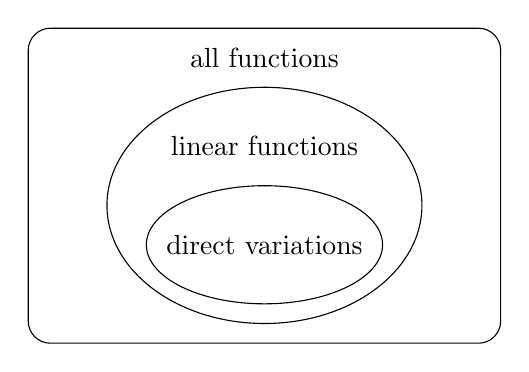
\begin{tikzpicture}
	\draw[rounded corners=8pt] (0,0) rectangle (6,4);
	\draw (3,3.625) node {all functions};
	\draw (3,1.75) circle[x radius=2cm, y radius=1.5cm];
	\draw (3,2.5) node {linear functions};
	\draw (3,1.25) circle[x radius=1.5cm, y radius=0.75cm];
	\draw (3,1.25) node {direct variations};
\end{tikzpicture}
\end{center}

Every direct variation is a linear function, but not every linear function is a direct variation. What makes direct variation ``special''?

\subsubsection{Graph of direct variation}

This is the easiest way to spot a direct variation. It must be a straight line that goes through the origin. That's it, really! Since every direct variation is of the form $y=kx$, it's quite easy to see that when $x=0$, we have $y = k\cdot0 = 0$. So the point $(0,0)$ is always on the graph of a direct variation. This makes sense in the context of the startup exploration: if Yeardleigh exchanges 0 dollars, she gets back 0 rupees.

\subsubsection{Equation of direct variation}

The equation of a direct variation will be of the form $y = kx$. It seems simple enough, but trickiest thing that might come up here is if we encounter an equation which, at first glance, doesn't appear to be a direct variation but which, with a little manipulation (using the POEs), can be transformed into a direct variation.

\begin{boxex}
Which of the following rules show that $x$ and $y$ are directly proportional? If a rule is a direct variation, state the constant of variation.

\begin{center}
\begin{minipage}{0.4\linewidth}
(a)~ $\dfrac{y}{x} = \dfrac{1}{2}$

(c)~ $y + 7 = 2x + 4$
\end{minipage}
%
\begin{minipage}{0.4\linewidth}
(b)~ $2y = 8x$

(d)~ $3y + 1 = x + 1$
\end{minipage}
\end{center}

\exsoln\ Equations (a), (b), and (d) represent direct variation; equation (c) does not. Equation (a) is clearly a direct variation with $k = \frac{1}{2}$. With equation (b) we can use DPOE to divide both sides by 2. The result is an equation of the form $y=4x$, and that's another direct variation with $k=4$.

With equation (c) we can use SPOE to get $y$ by itself, but the result is $y = 2x-3$, and this is not a direct variation. When we isolate $y$ with equation (d) --- first using SPOE and then DPOE --- we have $y = \frac{1}{3}x$. That's a direct variation with $k=\frac{1}{3}$.
\end{boxex}

The lesson here is: if we can transform and equation using the POEs into and equation of the form $y = kx$, then we have a direct variation.

\subsubsection{Data table of direct variation}

Up until this point, we have studied techniques for identifying a table of data (or a sequence) as linear, exponential, or quadratic. We've always been given tables that count sequentially through $x$-values $(0, 1, 2, 3, \dotsc)$. As we study the different types of functions in more depth, we will be able to identify functions from tables which aren't sequential, or which jump around.

For directly proportional relationships, we should be able to recognize not just that they are ``linear'', but that they are specifically ``direct variation''. The test for a direct variation goes back to the defining characteristic of a direct variation: the fact that $\frac{y}{x}$ is constant.

\begin{boxex}
Do the following data tables show direct variation? If so, write the equation for the direct variation.
\begin{center}
\begin{minipage}{0.4\linewidth}
\centering
(a)\par\begin{tabular}{|C{1cm}|C{1cm}|}
\hline
x & y\\\hline
-7 & 21\\
9 & -27\\
13 & -39\\\hline
\end{tabular}
\end{minipage}
%
\begin{minipage}{0.4\linewidth}
\centering
(b)\par\begin{tabular}{|C{1cm}|C{1cm}|}
\hline
x & y\\\hline
40 & 10\\
16 & 64\\
-20 & -5\\\hline
\end{tabular}
\end{minipage}
\end{center}

\exsoln\ Table (a) shows a direct variation, since for each line of the table, we have the same ratio: \[\frac{y}{x} = \frac{21}{-7} = \frac{-27}{9} = \frac{-39}{13} = -3\] The equation for this direct variation is $\frac{y}{x} = -3$ or $y = -3x$.

Table (b) does not represent a direct variation. The first and last rows have the same ratio, but the ratio of the middle row is different: \[\frac{10}{40} = \frac{-5}{-20} = \frac{1}{4} \quad\text{but this is different from}\quad \frac{64}{16} = 4\]
\end{boxex}

The ratio $\frac{y}{x}$ has to be the same for all points, otherwise we do not have a direct variation. This is one of the things that makes a direct variation special. A table can still be linear and not be a direct variation: there are lots of straight lines that \textit{do not} go through the origin! In \cref{ch:linear} we will learn a different way to determine whether a table of data represents a (generic) linear function.

Here's one more example of the kind of question we might encounter about direct variation.

\begin{boxex}
Find the missing value in each case: (a) A direct variation includes the points $(16, -2)$ and $(x, 4)$. Determine the value of $x$. (b) A different direct variation includes the points $(6, 30)$ and $(-10, y)$. Determine the value of $y$.

\exsoln\ We are told that we have a direct variation, and so we know that the two points must share the same ratio. We can therefore set up a proportion to solve part (a):
\[\frac{-2}{16} = \frac{4}{x}\] and solve to find the value of $x$. We find that $x=-32$.

Let's use a different approach to solve part (b). Knowing one point is enough to write the equation for the direct variation. We know that the point $(6,30)$ is on the direct variation, and so \[k = \frac{y}{x} = \frac{30}{6} = 5.\] Therefore, we have the equation $y = 5x$. We can then substitute $-10$ for $x$ and solve to discover that $y=-50$.
\end{boxex}

A final note: Technically, we can write all of these ratio with $x$ over $y$ and find the answers we are looking for. The reason we stick so closely to ``$y$ over $x$'' is the relationship that this quantity has to the unit rate in the problem. Plus, we want the notation that we use with direct variations to be consistent with the notation we use with linear functions generally.\footnote{We will meet a very important ratio called \textit{rate of change} in the next chapter. In this ratio we set the change in the independent variable over the change in the dependent variable.}

\addtodoitem{Graphs and  visuals for DV}


% % % % % % % % % % % % % % % % % % % % % % % % % % % % % % % % % % % % % % % % 
\section{Inverse variation}
\label{sec:inversevar}

%\begin{boxexplore}[Extended exploration: Teeter totter nickels]
%\addtodoitem{Click here to visit the extended exploration: Teeter Totter Nickels}
%\end{boxexplore}
\addtodoitem{Link to extended exploration: Teeter-totter nickels}

\begin{boxexplore}[Herb garden]
Fran\c{c}ois has enough mulch to plant an herb garden covering 24 square meters. Plus, he has whole barn full of snap-together fencing units that are each 1-meter long. How many different herb gardens can Fran\c{c}ois create, if he wants to use all the mulch and surround the garden with a rectangular fence?
\end{boxexplore} %% End of startup exploration

\kverse{Francois plants an herb garden.}

To solve Fran\c{c}ois's problem, we need to find a rectangle that has natural number side lengths and whose area is 24 square meters. One candidate is the long, skinny rectangle that is 1 meter by 24 meters. Of course, that's not the only one! We list the possible rectangles below and plot a graph of the data.

\begin{minipage}[c]{0.4\textwidth}
	\centering
	\begin{tabular}{|C{2cm}|C{2cm}|}
	\hline
	\text{\footnotesize Length ($x$)} & \text{\footnotesize Width ($y$)}\\\hline
	1 & 24\\
	2 & 12\\
	3 & 8\\
	4 & 6\\
	6 & 4\\
	8 & 3\\
	12 & 2\\
	24 & 1\\\hline
	\end{tabular}
\end{minipage}
%
\begin{minipage}[c]{0.6\textwidth }
	\centering
	\resizeplot{0}{0}{24}{24}
	\begin{tikzpicture}
		\begin{axis}[
			standard,
			xlabel={Length},
			ylabel={Width},
			minor xtick={0,...,24},
			minor ytick={0,...,24},
			xlabel near ticks,
			ylabel near ticks,
			width=1\linewidth,		% size
			height=1\linewidth,		% size
		]
			\addplot[algpoints, green!60!black] coordinates {(1,24)(2,12)(3,8)(4,6)(6,4)(8,3)(12,2)(24,1)};
		\end{axis}
	\end{tikzpicture}
%	\begin{tikzpicture}[scale=0.325]
%		%% grid setup
%		\draw[very thin, color=gray!25] (0,0) grid (24, 24);
%		\draw[->,thick] (0,0) -- (24,0); % node[right]{$x$-axis};
%		\draw[->,thick] (0,0) -- (0,24); % node[above]{$y$-axis};
%		\foreach \x in {0,2,...,24} \draw (\x,0.05) -- (\x,-0.05) node[below] {\footnotesize\x};
%		\foreach \y in {0,2,...,24} \draw (-0.05,\y) -- (0.05,\y) node[left] {\footnotesize\y};
%		%% points
%		\draw[green!60!black] plot[only marks, mark=*, mark size=8] coordinates {(1,24)(2,12)(3,8)(4,6)(6,4)(8,3)(12,2)(24,1)};
%	\end{tikzpicture}
\end{minipage}

The first thing that should jump out about this graph is that it is definitely not linear! The J-like shape suggests that it could be an exponential relationship\ldots\ but is it? What could we do to determine whether or not this is an exponential relationship?

\begin{boxwarn}[Full disclosure]
Even though we're beginning our discussion of linear functions, inverse variation is \textit{not} a linear relationship. We discuss it here just as a way to compare and contrast inverse and direct variation.
\end{boxwarn}

\begin{boxdef}[Inverse variation]
The variables $x$ and $y$ are said to be \textit{inversely proportional} if their values have a constant product. In other words, $xy = k$, where $k$ is a constant called the \textit{constant of variation}.

An equation of the form $y = \frac{k}{x}$ is called an \textit{inverse variation}. The quantities $x$ and $y$ are inversely proportional.
\end{boxdef}

In an inverse variation (where the variables are inversely proportional), the most important thing to remember is the fact that $x \cdot y$ is constant. For every point $(x, y)$ the product of $x$ and $y$ is always the same number.

When we force the product of two numbers to be the same, certain patterns arise. Most notably, if the value of one of the quantities goes up, the other one has to go down.

%Balancing a Teeter-Totter (See-saw) or Mobile
%Another related example deals with balancing a teeter-totter or mobile. If you have two objects balancing on a teeter-totter, the heavier object has to sit closer to the center. The lighter object has to be further from the center in order for things to balance. Now, it so happens that the relationship between distance from fulcrum and weight is more specific than ``less weight requires greater distance.''
%
%In class, we created some incredibly cheap teeter-totters out of rulers and pencils, and balanced them using nickels. In the course of the activity, you would have noticed that weight * distance on the left side had to equal weight * distance on the right side in order for things to balance. Weight * Distance was constant to achieve balance. We can turn these observations into an equation.
%Assume that WL = weight on left side, WR = weight on right side, DL = distance on left side, and DR = distance on right side. WL * DL = WR * DR
%Note: Balancing a mobile works exactly the same way and is the premise behind a problem solving technique called mass point geometry.

\subsubsection{Data table of inverse variation}

If we step away from context and think purely about data, the test for whether some data shows an inverse variation is whether $xy = k$, some constant value.

\begin{boxex}
Do the tables below show inverse variation? If so, write the equation for the direct variation.
\begin{center}
\begin{minipage}{0.4\linewidth}
\centering
(a)\par\begin{tabular}{|C{1cm}|C{1cm}|}
\hline
x & y\\\hline
2.5 & 20\\
-10 & -5\\
8 & 5.5\\\hline
\end{tabular}
\end{minipage}
%
\begin{minipage}{0.4\linewidth}
\centering
(b)\par\begin{tabular}{|C{1cm}|C{1cm}|}
\hline
x & y\\\hline
3.5 & 4\\
1 & 14\\
-7 & -2\\\hline
\end{tabular}
\end{minipage}
\end{center}

\exsoln\ Table (a) does not represent an inverse variation. The first and second rows of the table have the same product (50), but the last row has a different product (44) Table (b) does represent an inverse variation: all three rows have the same product (14). So, table (b) has equation $xy = 14$.
\end{boxex}

\begin{boxex}
Find the missing values in the table, given that the data represent an inverse variation.
\begin{center}
(a)\par\begin{tabular}{|C{1cm}|C{1cm}|}
\hline
x & y\\\hline
3 & a\\
9 & 4\\
2 & b\\
c & 8\\\hline
\end{tabular}
\end{center}

\exsoln\ The second row of the table gives us the clue we need: $9\cdot4 = 36$, so that must be the constant of variation for this inverse variation. Then, it is simply a matter of finding the partner of each value that multiplies to get 36.

In the first row, $3a = 36$ implies that $a=12$. In the third row, $2b=36$ implies that $b=18$. In the fourth row, $8c=36$ implies that $c=4.5$.
\end{boxex}

\subsubsection{Equation of inverse variation}

We have seen that the equation for an inverse variation is either $yx = k$ or $y=\frac{k}{x}$. Writing the equation for an inverse variation brings out two important features that we must be aware of. Consider the equation \[y = \frac{k}{x}\]

First, what happens when $x=0$? Yikes! Remember, division by zero is undefined, and so 0 is an illegal value for $x$. We say that 0 must be \textit{restricted from the domain} of the function.

Second, what happens when $y=0$\ldots\ or is that even possible? Note that as $x$ gets larger and larger, the value of the fraction $1/x$ gets smaller and smaller (closer and closer to zero). But, no matter how big $x$ gets, $1/x$ will never be \textit{equal to} zero. It will get close to zero. Super close! Impossibly close! But it will never equal zero.

We can see this unusual behavior reflected in the graph.

\addtodoitem{asymptote in I.V. section}

\subsubsection{Graph of inverse variation}

Not being able to have an $x$ or $y$ value of zero does very interesting things to the graphs. Consider the inverse variation $xy=12$ or $y = \frac{12}{x}$:

\resizeplot{-12}{-12}{12}{12}
\begin{center}
\begin{tikzpicture}
	\begin{axis}[standard]
		\addplot[algcurve, green!50!black, domain=-12:-1] (\x,12/\x);
		\addplot[algcurve, green!50!black, domain=1:12] (\x,12/\x);
%		\draw[red] (axis cs:1.5,1,0) node[right]{\large$y=5x-6$};
%		\addplot[algpoints, red] coordinates {(-5,-22)(-4,-17)(-3,-12)(-2,-7)(-1,-2)(0,3)(1,8)(2,13)(3,18)(4,23)(5,28)};
	\end{axis}
\end{tikzpicture}
\end{center}

%\begin{center}
%	\begin{tikzpicture}[scale=0.4]
%		%% grid setup
%		\draw[very thin, color=gray!25] (-12,-12) grid (12, 12);
%		\draw[->,thick] (-12,0) -- (12,0); % node[right]{$x$-axis};
%		\draw[->,thick] (0,-12) -- (0,12); % node[above]{$y$-axis};
%		\foreach \x in {-12,-10,...,12} \draw (\x,0.05) -- (\x,-0.05) node[below] {\footnotesize\x};
%		\foreach \y in {-12,-10,...,12} \draw (-0.05,\y) -- (0.05,\y) node[left] {\footnotesize\y};
%		%% points
%		\draw[<->, very thick, blue, domain=-12:-1] plot (\x,12/\x);
%		\draw[<->, very thick, blue, domain=1:12] plot (\x,12/\x);
%	\end{tikzpicture}
%\end{center}

Notice a few things: First, we can see from the graph that this is not an exponential relationship. Although the portion of the graph in the first quadrant might look exponential, when we plug in negative input values we get different behavior that we'd expect from an exponential.

Secondly, the graph is in two disconnected pieces, and since it never crosses the $x$- or $y$-axis, it appears entirely in the first and third quadrants. It appears in those particular quadrants because of the defining feature of inverse variation: $x$ and $y$ have a constant product.

This graph is the picture of all points whose coordinates have a product of (positive) 12. The only way to get a positive product is to either multiply two positive numbers, or two negative numbers --- exactly the description of the coordinates in the first and third quadrants! What do you suppose the graph of $y=\frac{-12}{x}$ might look like?

\begin{boxex}
Write the equation for the inverse variation pictured in the graph below.

\resizeplot{-7}{-7}{7}{7}
\begin{center}
\begin{tikzpicture}
	\begin{axis}[
			standard,
			minor xtick={-7,...,7},
			minor ytick={-7,...,7},
		]
		\addplot[algcurve, blue, domain=-6.5:-0.85] (\x,-6/\x);
		\addplot[algcurve, blue, domain=0.85:6.5] (\x,-6/\x);
%		\draw[red] (axis cs:1.5,1,0) node[right]{\large$y=5x-6$};
		\addplot[algpoints, blue] coordinates {(-2,3)(-3,2)(3,-2)(2,-3)(-1,6)(1,-6)(6,-1)(-6,1)};
	\end{axis}
\end{tikzpicture}
\end{center}

%\begin{center}
%	\begin{tikzpicture}[scale=0.65]
%		%% grid setup
%		\draw[very thin, color=gray!25] (-7,-7) grid (7, 7);
%		\draw[->,thick] (-7,0) -- (7,0); % node[right]{$x$-axis};
%		\draw[->,thick] (0,-7) -- (0,7); % node[above]{$y$-axis};
%		\foreach \x in {-7,...,7} \draw (\x,0.05) -- (\x,-0.05) node[below] {\footnotesize\x};
%		\foreach \y in {-7,...,7} \draw (-0.05,\y) -- (0.05,\y) node[left] {\footnotesize\y};
%		%% points
%		\draw[<->, very thick, blue, domain=-6.5:-0.85] plot (\x,-6/\x);
%		\draw[<->, very thick, blue, domain=0.85:6.5] plot (\x,-6/\x);
%		\draw[blue] plot[only marks, mark=*, mark size=4] coordinates {(-2,3)(-3,2)(3,-2)(2,-3)(-1,6)(1,-6)(6,-1)(-6,1)};
%	\end{tikzpicture}
%\end{center}

\exsoln\ Since we know that this is an inverse variation, all we need is to find the coordinates of one point. Some are plotted for us, so that's good news. If we use the point $(-2, 3)$, we can see that $k = xy = -2\cdot3 = -6$. Once we have found the constant of variation, we can easily write the equation: $xy=-6$ or $y=\frac{-6}{x}$.
\end{boxex}

\subsubsection{About the ``family'' of inverse variation}

You may have noticed that inverse variation doesn't seem to fit into any of the function families we have looked at so far. This is true. Inverse variation doesn't belong to linear, quadratic, exponential families of functions, and so we won't do much more with inverse variation for quite a while.

Inverse variation is actually a member of the super-family of functions called \textit{rational functions}, which is more of a focus in Algebra 2. This rational super-family has a number of interesting and surprising features, and they can take on a whole variety of bizarre shapes.

Inverse variation graphs do have something in common with exponential functions: asymptotes. As we saw, inverse variations get impossibly close to both the $x$- and $y$-axis, but never reach them. Generally, these graphs have two asymptotes, one horizontal, one vertical.

% % % % % % % % % % % % % % % % % % % % % % % % % % % % % % % % % % % % % % % % 
\chaptersummary

In this chapter we started in familiar territory: writing and solving proportions. We quickly progressed into a more ``algebraic zone'', though, by extending the idea of proportionality to the idea of variation.

We also saw how a directly proportional relationship gives rise to a linear function: the direct variation. We'll take this idea and run with it in the next chapter: Why should we be limited to straight lines that go through the origin, when we can learn to desrcibe straight lines in general? Onward!
